\documentclass[10pt,twoside,a4paper,fleqn]{report}

\usepackage{braket}
\usepackage{graphicx}
\usepackage{parskip}
\usepackage{amssymb}
\usepackage{mathbbol}
\usepackage{enumerate}
\usepackage{ragged2e}
\usepackage{eurosym}
\usepackage{amsmath}

% Defining some new mathematics commands
\newcommand*{\colvec}[1]{\begin{pmatrix}#1\end{pmatrix}}
\newcommand*{\0}{$\ket{0}$}
\newcommand*{\1}{$\ket{1}$}

\usepackage[english,bt]{ethidsc} % Special IDSC styles and commands      	
\usepackage{apacite}
								 % {german}/english: language of headings, etc.
								 % {st}/bt/mt: {semester}/bachelor/master thesis
							
% Page header (don't change)____________________________________________________
\setlength{\parindent}{0em}                 % Disable parindent
\rhead[\nouppercase{\rightmark}]{\thepage}  % Special headings
\lhead[\thepage]{\nouppercase{\leftmark}}   % Special headings
\cfoot{}                                    % Special headings


% Title page (please fill in)___________________________________________________
\title{Quantum Machine Learning}


\studentA{Mark Fingerhuth}
\ethidA{I6082973}
\semesterA{5}
\emailA{m.fingerhuth@student.maastrichtuniversity.nl}

%\studentB{Second Student}
%\ethidB{12-345-678}
%\semesterB{9}
%\emailB{second@student.ethz.ch}

\supervision{Prof. Francesco Petruccione\\ Dr. Fabrice Birembaut}
\date{January 2017}

\identification{IDSC-XX-YY-ZZ} 		% Project identifier

%\infopage %includes the last page
%\declaration

% Begin document________________________________________________________________
\begin{document}

\maketitle 							% Create title page


% Preamble______________________________________________________________________

\pagenumbering{roman} 				% Begin roman page numbering (i,ii,...)

%---------------------------------------------------------------------------
% Preface

\chapter*{Preface}

Blah blah \dots

 \cleardoublepage

%---------------------------------------------------------------------------
% Table of contents

 \setcounter{tocdepth}{2}
 \tableofcontents

 \cleardoublepage

%---------------------------------------------------------------------------
% Abstract

\chapter*{Abstract}
 \addcontentsline{toc}{chapter}{Abstract}

NEEDS MODIFICATION!

Quantum machine learning, the intersection of quantum computation and classical machine learning,
bears the potential to provide more efficient ways to deal with big data through the use of quantum
superpositions, entanglement and the resulting quantum parallelism. The proposed research will
attempt to implement and simulate two quantum machine learning routines and use them to solve
small machine learning problems. That will establish one of the earliest proof-of-concept studies in
the field and demonstrate that quantum machine learning is already implementable on small-scale
quantum computers. This is vital to show that an extrapolation to larger quantum computing devices
will indeed lead to vast speed-ups of current machine learning algorithms.

 \cleardoublepage

%---------------------------------------------------------------------------
% Symbols

\chapter*{Nomenclature}\label{chap:symbole}
 \addcontentsline{toc}{chapter}{Nomenclature}

\section*{Symbols}
\begin{tabbing}
 \hspace*{1.6cm} \= \hspace*{8cm} \= \kill
 $\otimes$ \> Tensor product \\[0.5ex]
 $i$ \> Imaginary unit \> $i=\sqrt{-1}$ \\[0.5ex]
 $\dagger$ \> Hermitian conjugate \> Complex conjugate transpose \\[0.5ex]
 $!$ \> Factorial \> e.g. 3! = 3*2*1 \\[0.5ex]
\end{tabbing}

\section*{Indicies}
\begin{tabbing}
 \hspace*{1.6cm}  \= \kill
 a \> Ambient \\[0.5ex]
 air \> Air
\end{tabbing}

\section*{Acronyms and Abbreviations}
\begin{tabbing}
 \hspace*{1.6cm}  \= \kill
 QML \> Quantum machine learning \\[0.5ex]
 QC \> Quantum computer \\[0.5ex]
 Prob \> Probability \\[0.5ex]
 PM \> Post-measurement \\[0.5ex]
 HD \> Hamming distance \\[0.5ex]
 CM \> Conditional measurement \\[0.5ex]
 CNOT \> Controlled NOT gate \\[0.5ex]
 CCNOT \> Controlled controlled NOT gate (Toffoli gate) \\[0.5ex]
 CU \> Controlled U gate (where U can be any unitary quantum gate) \\[0.5ex]
\end{tabbing}

 \cleardoublepage

%---------------------------------------------------------------------------


% Chapters______________________________________________________________________

\pagestyle{fancy}               	% Fancy headings
\pagenumbering{arabic}				% Begin arabic page numbering (1,2,...)

\chapter{Introduction}\label{sec:introduction}

The ability to recognise familiar faces, to understand spoken language and to distinguish types of vegetables comes naturally to humans, although these processes of pattern recognition and classification are inherently complex. Machine learning (ML), a subdiscipline of artificial intelligence, is concerned with the development of algorithms that perform these types of tasks, thus enabling computers to find and recognise patterns in data and classify unknown inputs based on previous training data. Such algorithms make the core of e.g. human speech recognition and recommendation engines as used by Amazon \cite{graves2013speech,linden2003amazon}.
% and algorithms that can predict heart disease from real-time electrocardiograms \citep{acharya2015integrated, pazzani2007content}.

According to \citeA{bigdata}, approximately 2.5 quintillions (${10}^{18}$) bytes of digital data are created every day. This growing number implies that many areas dealing with data will eventually require advanced algorithms that can make sense of data content, retrieve patterns and reveal correlations. However, most ML algorithms involve the execution of computationally expensive operations and doing so on large data sets inevitably takes a lot of time \cite{bekkerman2011scaling}. Thus, it becomes increasingly important to find efficient ways of dealing with big data.
%and/or reduce the computational complexity of the algorithms.

A promising solution is the use of quantum computation which has been researched intensively in the last few decades. Quantum computers (QCs) use quantum mechanical systems and their unique properties to manipulate and process information in ways that are impossible for classical computers. Analogous to a classical computer manipulating bits, a quantum computer makes use of so-called quantum bits (qubits). Bits and qubits are both binary entities meaning they can only take the values 0 and 1. However, a non-probabilistic classical bit can only take one of these values at a time whereas a qubit can also be found in a linear superposition of the two states.

%\begin{equation}
%\label{equ: simplequbit}
%\ket{q} = \alpha \ket{0} + \beta \ket{1}
%\end{equation}
%where $\alpha$ and $\beta$ are complex numbers and often referred to as amplitudes. When measuring qubit $\ket{q}$ it will take the value \0 with a probability of ${|\alpha|}^{2}$ and \1 with a probability of ${|\beta|}^{2}$. Since the total probability has to sum to unity, the normalization condition ${|\alpha|}^{2} + {|\beta|}^{2} =  1$ must be satisfied at all times.

This property gives rise to quantum parallelism, which enables the execution of certain operations on many quantum states at the same time. Despite this advantage, the difficulty in quantum computation lies in the retrieval of the computed solution since a measurement of a qubit collapses it into a single classical bit and thereby destroys information about its previous superposition. Several quantum algorithms have been proposed that provide exponential speed-ups when compared to their classical counterparts with Shor's prime factorization algorithm being the most famous \cite{shor1994}.
%As another example, Grover's quantum database search algorithm enables finding a single element in a list of $N$ elements within roughly $\sqrt{N}$ quantum mechanical steps instead of $N$ classical steps \citep{grover}.
Thus, quantum computation has the potential to improve computational power, speed up the processing of big data and possibly solve certain problems that are practically unsolvable on classical computers e.g. computationally-exhaustive optimisation problems such as the well-known travelling salesman problem with more than 1000 cities \cite{kieu2006quantum}.

%for the QML toolbox to be complete a quantum algorithm to solve systems of linear equations is needed since most ML algorithms rely on solving those.

Considering these advantages, the combination of quantum computation and classical ML into the new field of quantum machine learning (QML) seems almost natural. More specifically, one speaks of quantum-enhanced machine learning when quantum computation is used to improve classical ML algorithms. Yet, both fields are mutually beneficial to each other since classical ML can also be used to improve aspects of quantum computation. For example, \citeA{las2016genetic} showed that a classical genetic algorithm can be used to reduce the experimental error in quantum logic gates. However, this thesis will only focus on the field of quantum-enhanced machine learning.

%There are currently two main ideas on how to merge quantum computation with ML, namely a) running the classical algorithm on a classical computer and outsourcing only the computationally intensive task to a QC or b) executing the quantum version of the entire algorithm on a QC. Current QML research mostly focusses on the latter approach by developing quantum algorithms that tap into the full potential of quantum parallelism.

\section{Motivation}
\label{sec:motivation}

Classical ML is a very practical topic since it can be directly tested, verified and implemented on any commercial classical computer. So far, QML has been of almost entirely theoretical nature since the required computational resources are not yet in place. To yield reliable solutions QML algorithms often require a huge number of error-correcting qubits and some quantum data storage such as the proposed quantum random access memory (qRAM) \cite{qRAM}. However, to date the maximum number of e.g. superconducting qubits reportedly used for calculation is nine, the D-Wave II quantum annealing device delivers 1152 qubits but can only solve a narrow class of problems, and a qRAM has not been developed yet \cite{hydrogensimulation, dwave2}. Furthermore, qubit error-correction is still a very active research field, and most of the described preliminary QCs deal with non-error-corrected qubits with short lifetimes and are, thus, impractical for large QML implementations.

Until now there have been only a few experimental verifications of QML algorithms that establish proof-of-principle. \citeA{Li2015} successfully distinguished handwritten digits using a quantum support vector machine on a four-qubit nuclear magnetic resonance test bench. In addition, \citeA{Cai2015} were first to experimentally demonstrate quantum machine learning on a photonic QC and showed that the distance between two vectors and their inner product can indeed be computed quantum mechanically. Lastly, \citeA{Riste2015} solved a learning parity problem with five superconducting qubits and found that a quantum advantage can already be observed in non-error-corrected systems.

%Consequently,
Considering the gap between the number of proposed QML algorithms and the few experimental realisations, it becomes important to find QML problems which can already be implemented on small-scale QCs. Hence, the purpose of this research is to provide proof-of-principle implementations and simulations of selected QML algorithms on small datasets. For this purpose, the $k$-nearest neighbour algorithm, one of the simplest ML algorithms, was chosen as a good minimal example for implementation and quantum simulation. This is a necessary step in the attempt to shift QML from a purely theoretical research area to a more applied field such as classical ML.

\section{Research question}
\label{sec:researchquestion}


%Don't know where this should go!

%Matthias Troyer citation for this part:

%Finding optimal ways of compiling a given quantum algorithm as well as designing a high-level programming language or environment similar to that of classical computer code editors is called \emph{quantum software engineering}.

In light of the theoretical nature of current QML research and the small number of experimental realisations, this research will address the following question:

%NARROW DOWN THE RESEARCH QUESTION!
\centering\textbf{How can a k-nearest neighbour quantum machine learning algorithm be implemented on small-scale quantum computers?}

%Alternatives:
%Is it possible to experimentally demonstrate that two QML algorithms proposed by \cite{Schuld2014, Schuld2016} can already solve a small ML problem using classical simulation or IBMs quantum processor?
%Is it possible to already implement and solve a small ML problem on IBMs publicly available quantum computer?

\justify
The following sections will introduce the necessary theoretical foundations, and the tools used to answer this research question. 

\cleardoublepage
%\chapter{Materials and Methods}\label{sec:materialsandmethods}
%\cleardoublepage
%\chapter{Results and Discussion}\label{sec:resultsanddiscussion}


\subsubsection{Diffusion matrix from quantum random walks}
\label{subsubsubsec:diffusion}

For the simplest case, consider the entries in the classical probability vector v to be normal distributed, e.g.

CHECK THE ORDER!
\begin{equation}
v = \colvec{0.064180\\0.146860\\0.146770\\0.341590\\0.026840\\0.063590\\0.061700\\0.148470}
\end{equation}

The goal is to encode this classical data into a quantum memory state $\ket{M}$ of the form,

\begin{align}
\ket{M} = \quad &0.064180 \ket{000} +
0.146860 \ket{100} +
0.146770 \ket{010} +
0.341590 \ket{001}\notag\\
&+ 0.026840 \ket{110}
+ 0.063590 \ket{011} +
0.061700 \ket{101} +
0.148470 \ket{111}
\end{align}

%Before outlining how to prepare state $\ket{M}$ the notion of Hamming distance needs to be introduced.

Furthermore, a useful tool of visualizing the HDs between binary patterns made from three qubits is a 3-D cube as shown in Fig.~\ref{img:cubenoprobs}. On the cube, adjacent qubit patterns have a HD of 1 and the HD increases by 1 for every additional corner. For example, the qubit state $\ket{000}$ is adjacent to $\ket{100}$ since they only differ in one qubit ($HD=1$). Moving one more corner yields the state $\ket{101}$ or $\ket{110}$ which both have a HD of 2 compared to $\ket{000}$.

\begin{figure}[!ht]
       \centering
       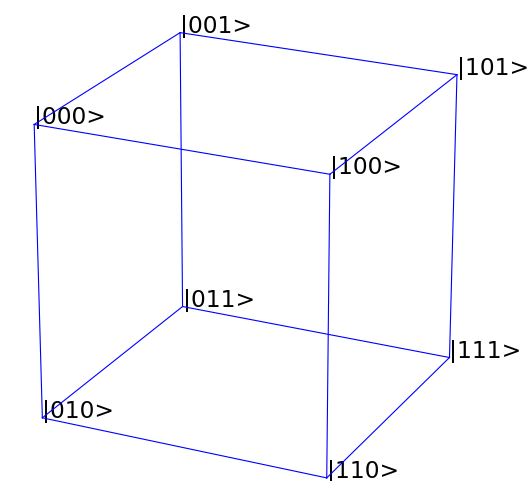
\includegraphics[width=0.5\textwidth]{img/cubewithoutprobs.png}
       \caption{\label{img:cubenoprobs} Visualizing Hamming distances on a 3-D cube}
\end{figure}

This way of visualizing HDs can be extended to the 16 binary patterns made by four qubits that can be visualized on a 4-D cube, also called tesseract, as illustrated in Fig.~\ref{img:hypercubenoprobs}.

\begin{figure}[!ht]
       \centering
       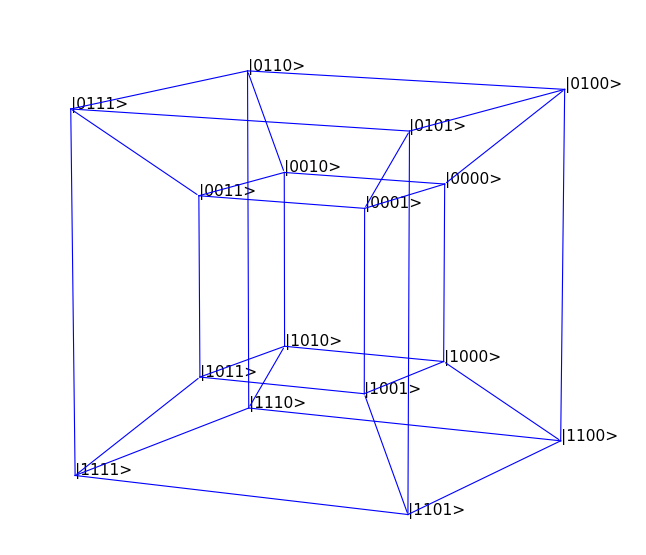
\includegraphics[width=0.5\textwidth]{img/hypercubewithoutprobs.png}
       \caption{\label{img:hypercubenoprobs} Visualizing Hamming distances on a 4-D cube (tesseract)}
\end{figure}

The idea of a coin operator $C$ can be borrowed from the theory of quantum random walks to initialize a gaussian distribution centered around a chosen binary qubit pattern. For this purpose, the coin operator is defined as,

\begin{equation}
C = \begin{pmatrix}
\sqrt{\delta} & 1-\sqrt{\delta} \\
1-\sqrt{\delta} & -\sqrt{\delta}
\end{pmatrix}
\end{equation}

where $0 \leq \delta \leq 1$.


\subsubsection{Amplitude-based quantum kNN algorithm}
\label{subsubsubsec:quantumknearestneighbouramplitudes}

\begin{equation}
\frac{1}{\sqrt{2M}}\sum_{m=1}^{M} (\textcolor{emerald}{\ket{0}}\ket{\textcolor{red}{\Psi_{\tilde{x}} (\star)}}+\textcolor{emerald}{\ket{1}}\ket{\textcolor{darkyellow}{\Psi}_{\textcolor{purple}{x^{m}}}})\ket{y^{m}(\textcolor{darkyellow}{A} \ or \ \textcolor{purple}{B})}\ket{m}
\end{equation}
where
\begin{equation}
\ket{\textcolor{red}{\Psi_{\tilde{x}} (\star)}} = \sum_{i=1}^{N} \textcolor{red}{\tilde{x}_i}\ket{i} \quad \quad
\ket{\textcolor{darkyellow}{\Psi}_{\textcolor{purple}{x^{m}}}}	 = \sum_{i=1}^{N} \textcolor{darkyellow}{x}\textcolor{purple}{_i^m} \ket{i} 
\end{equation}

\begin{equation}
e.g. \quad \begin{pmatrix}
 \textcolor{blue}{0.6} \\ 
 \textcolor{emerald}{0.4}
 \end{pmatrix} \quad \rightarrow \quad \ket{n} =  \sqrt{\textcolor{blue}{0.6}}\ket{0}+\sqrt{\textcolor{emerald}{0.4}}\ket{1}
\end{equation}

Applying the \textbf{Hadamard gate} interferes the input and the training vectors:

\begin{equation}
\frac{1}{2\sqrt{M}}\sum_{m=1}^{M} (\textcolor{emerald}{\ket{0}}[\ket{\textcolor{red}{\Psi_{\tilde{x}}}}+\ket{\textcolor{darkyellow}{\Psi}_{\textcolor{purple}{x^{m}}}}]+\textcolor{emerald}{\ket{1}}[\ket{\textcolor{red}{\Psi_{\tilde{x}}}}-\ket{\textcolor{darkyellow}{\Psi}_{\textcolor{purple}{x^{m}}}}])\ket{y^{m}(\textcolor{darkyellow}{A} \ or \ \textcolor{purple}{B})}\ket{m}
\end{equation}

$\rightarrow$ Perform \textbf{conditional measurement} on ancilla qubit.\\
Successful if $\ket{0}$ state is measured.

After successful conditional measurement, the state is proportional to
\begin{equation}
\frac{1}{2\sqrt{M}}\sum_{m=1}^{M} \sum_{i=1}^{N} (\textcolor{red}{\tilde{x}_i}+\textcolor{darkyellow}{x}\textcolor{purple}{_i^m})\ket{0}\ket{i}\ket{y^{m}(\textcolor{darkyellow}{A} \ or \ \textcolor{purple}{B})}\ket{m}
\end{equation}

Probability to measure class B:
\begin{equation}
p(\ket{y^m} = \ket{1(\textcolor{purple}{B})})= \sum_{m \mid y^m=1(\textcolor{purple}{B})} 1 - \frac{1}{4M} \mid \textcolor{red}{\tilde{x}} - \textcolor{purple}{x^m} \mid ^2
\end{equation}

Hereby, the advantages of the quantum version are the parallel computation of the distances between each training vector and the input vector as well as contracting distance computation and distance weighting into one computational step.

The quantum advantage of the algorithm is the simultaneous computation of the HD between the input vector and each training vector which is impossible to do classically. For example, if the training set contains 1,000,000 vectors with 10 entries each, the quantum algorithm performs all 1,000,000 distance computations with the application of only 10 X and 10 CNOT gates. In contrast, the classical algorithm would need to perform  1,000,000 individual computations in order to be able to apply distance-dependent weights to each training vector. 


\subsubsection{Controlled U Gate}
\label{subsubsubsec:controlledugate}

Often there is a need for applying certain quantum gates in a controlled manner. Thus a controlled U (CU) gate is required whereby U can be any unitary single-qubit gate. The CU gate is defined as:

\begin{equation}
CU = \begin{pmatrix}
 \mathbb{1} & 0 \\ 
 0 & U
 \end{pmatrix}
\end{equation}

It is important to note that the CNOT gate is essentially a CU gate in the case of U = X. 

Most of the time the CU gate cannot be implemented directly and has to be realized through larger quantum circuits consisting of CNOT and single-qubit gates. \citeA{nielsen2010quantum} describe such a decomposition as shown in Fig.~\ref{img:cudecomposition}.

\begin{figure}[ht]
   \centering
   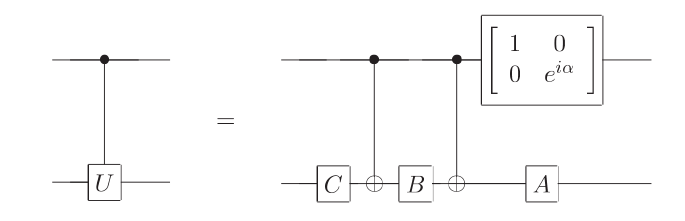
\includegraphics[width=0.7\textwidth]{img/controlledudecomp.png}
   \caption{Circuit decomposition for a controlled-U operation for single-qubit gate U.\textsuperscript{3}}
   \label{img:cudecomposition}
\end{figure}

\footnotetext[3]{Reprinted from Michael A. Nielsen and Isaac L. Chuang. Quantum Computation and Quantum Information. Cambridge University Press, 2000. Copyright 2010 by Nielsen \& Chuang.}

The idea is that when the control qubit is \0 the gate combination ABC is applied to the target qubit and has to equal the identity gate:

\begin{equation}
ABC = \mathbb{1}
\end{equation}

If and only if the control qubit is \1 then the gate sequence $e^{i\alpha}AXBXC$ is applied to the target. Since the goal is to apply the unitary U to the target qubit the following equation must be satified,

\begin{equation}
e^{i\alpha}AXBXC = U
\end{equation}

In order to find the matrices A,B,C and the additional parameter $\alpha$ the following equation has to be solved:

\begin{equation}
U = \begin{pmatrix}
 e^{i(\alpha-\frac{\beta}{2}-\frac{\delta}{2})}\cos{\frac{\gamma}{2}} & -e^{i(\alpha-\frac{\beta}{2}+\frac{\delta}{2})}\sin{\frac{\gamma}{2}} \\ 
e^{i(\alpha+\frac{\beta}{2}-\frac{\delta}{2})}\sin{\frac{\gamma}{2}} & e^{i(\alpha+\frac{\beta}{2}+\frac{\delta}{2})}\cos{\frac{\gamma}{2}}
 \end{pmatrix}
\end{equation}
%\cleardoublepage
%\chapter{Outlook}\label{sec:outlook}
%\cleardoublepage
%\chapter{Conclusion}\label{sec:conclusion}

Quantum-enhanced machine learning aims to harness the properties of quantum mechanical systems to enhance the performance of classical machine learning algorithms beyond the reach of classical computers. This becomes increasingly important since big data pushes computational resources and classical algorithms to their limits. This research established proof-of-principle simulations of two variants of a distance-weighted quantum $k$-nearest neighbour (kNN) algorithm using three small-scale supervised machine learning tasks.
%However, current quantum computing efforts have not yet led to the construction of a large-scale universal quantum computer and, thus, most of the current quantum-enhanced machine learning research is purely theoretical. Yet, small-scale quantum computers have been realised already and up to 30 qubits can still be simulated on a conventional laptop. Thus, this research is part of the attempt to shift quantum-enhanced machine learning into a more applied field by establishing proof-of-principle simulations of two variants of a distance-weighted quantum $k$-nearest neighbour (kNN) algorithm using three small-scale supervised machine learning tasks.
%On the other hand, IBM has enabled public access to their five-qubit quantum computer and small quantum computers with up to 30 qubits can still be simulated on conventional laptops. 

Firstly, the qubit-based kNN algorithm by \citeA{Schuld2014} was combined with a quantum state preparation routine by \citeA{Trugenberger2001} to classify various 9-bit RGB colours into the classes \emph{red} and \emph{blue}. Microsoft's software architecture Liqui$\ket{}$ was used to simulate the algorithm on two levels of difficulty. In the easy evaluation stage, the quantum kNN achieved a classification accuracy of 75\% which was subsequently raised to 100\% in the more challenging evaluation stage with a larger training dataset. These results show that the qubit-based kNN routine is a very effective classification algorithm concerning 9-bit RGB colours.

Aiming for an implementation with the IBM Quantum Experience, an amplitude-based kNN algorithm (aKNN) was developed by \citeA{SchuldFingerhuth}.  A simple binary Bloch vector classification tasks was considered to keep the requirements on the quantum hardware as small as possible. The necessary quantum compiling steps mapping the quantum state preparation routine and the aKNN algorithm to the IBM quantum hardware were outlined. For that particular classification task, it was shown that it could not be implemented within IBM's 40 quantum gate slots. Even though an implementation might be feasible using different datasets, the research demonstrated that there are cases which require relatively large gate sequences for implementation. As an alternative, the Bloch vector classification problem using the aKNN algorithm was simulated in Liqui$\ket{}$. The simulated algorithm led to the correct classification of two Bloch vectors. Lastly, the aKNN algorithm was simulated for the classification of discrete Gaussian distributions constituting a higher-dimensional classification problem using a slightly more advanced quantum state preparation routine. The simulated algorithm classified 83.3\% of various discrete Gaussian distributions correctly.

Overall, the Liqui$\ket{}$ quantum simulations clearly demonstrated the effectiveness of both quantum kNN algorithms. When combined with more general quantum state preparation routines, these algorithms bear the potential to speed up the processing of big data. Thus, a breakthrough in the development of a universal quantum computer would not solely constitute a major milestone in physics but most probably also revolutionise the field of machine learning.

%\cleardoublepage
%\chapter{Personal Reflection}\label{sec:personalreflection}

Personally, this bachelor thesis research has been instructive and beneficial in many different ways. Most importantly, I have had the opportunity to dedicate my entire time to learn about the subject of quantum information and, specifically, quantum machine learning in detail. Since these subjects are not taught within the curriculum of the Maastricht Science Programme (MSP) it was especially amazing to challenge myself to these notoriously difficult subjects within the intersection of quantum physics and computer science. In doing so, I have learned more about the methods of theoretical physics and gained additional experience in scientific programming with Octave, Python and F\#. Without prior knowledge of F\#, I was able to learn how to simulate quantum computations and quantum machine learning algorithms using the quantum simulation toolsuite Liqui$\ket{}$. Furthermore, I was able to use the first cloud-based quantum computer, the so-called IBM Quantum Experience, publicly released in May 2016 by IBM.

Alongside my research, I had the possibility to attend many great lectures, seminars and three conferences which were all generously funded by the Centre for Quantum Technology. This enabled me to get to know many renowned scientists working in the fields of quantum information, quantum machine learning, open quantum systems, quantum optics and quantum cryptography. Furthermore, I was provided with the opportunity to present my research at the 4\textsuperscript{th} South African conference for quantum information processing, communication and control in Cape Town in late November 2016. This constituted a big step with respect to my academic career and a great way of putting my acquired presentation skills to practice.

However, in retrospective I feel that I could have been more productive in office by structuring my work days more diligently. For example, the first one and a half months were mostly spent on reading research paper and text books to acquire the theoretical foundation for my research and little time was used to practice F\# within the Liqui$\ket{}$ framework. A possible solution for the future would be to divide each day into two parts: e.g. spending the morning with reading papers and books and the afternoon on practical work and programming. Besides this, I feel like I should have communicated my progress more with my internal supervisor Dr. Birembaut at the MSP.

In conclusion, the bachelor thesis research has showed me the importance of interdisciplinarity since the field of quantum information requires the understanding of concepts in computer science as well as quantum mechanics. Fortunately, MSP's liberal education does not only focus on textbook exercises and lectures but mostly teaches us how to systematically approach unknown topics and tackle problems therein. It was great to see that this enabled me to venture into a previously unfamiliar field and learn the necessary skills to conduct meaningful research. The newly acquired skills will certainly be useful for my planned masters in the field of quantum information.

%During the thesis work, I realized that encountering problem after problem is at the core of research but that one can resolve most of them when just showing enough dedication.

%The Centre for Quantum Technology at the University of KwaZulu-Natal in South Africa has been a wonderful host for my Bachelor thesis research. My supervisor Prof. Francesco Petruccione has become a mentor and friend and provided me with great opportunities for personal and academic growth. Furthermore, my collaborator Maria Schuld has shared vasts amount of knowledge, tricks and ideas with me and has always been a great help during my research work. Alongside my research, I had the possibility to attend many great lectures, seminars and three conferences which were all generously funded by the Centre for Quantum Technology. This enabled me to get to know many renowned scientists working in the fields of quantum information, quantum machine learning, open quantum systems, quantum optics and quantum cryptography. Attending the Quantum Machine Learning Workshop at the Dolphin Coast in July 2016 provided me with a broad overview of the field of quantum machine learning and was the first time that I ever attended a scientific conference. In November 2016, I was provided with the opportunity to present my research at the 4\textsuperscript{th} South African conference for Quantum Information Processing, Communication and Control in Cape Town. This opened the possibility for a collaboration with an experimental research group in Israel working on quantum computation with trapped ions. In January 2017, I am invited to the NiTheP Chris Engelbrecht Quantum Machine Learning Summer School where I will give three workshop sessions on quantum machine learning using the Liqui$\ket{}$ framework and the IBM Quantum Experience.
%\cleardoublepage
%\chapter{Working with \LaTeX\ }\label{sec:working}
This chapter explains how to typeset some of the most common elements contained in a technical report using \LaTeX.

\section{Headings}
Your report can be structured using several different types of headings. Use the commands \texttt{\textbackslash chapter\{.\}}, \texttt{\textbackslash section\{.\}}, \texttt{\textbackslash subsection\{.\}}, and \texttt{\textbackslash subsubsection\{.\}}. Use the asterisk symbol \texttt{*} to suppress numbering of a certain heading if necessary, for example, \texttt{\textbackslash section*\{.\}}.

\section{References and Footnotes}\label{sec:references}
References to literature are included using the command \texttt{\textbackslash
cite\{.\}}. For example \cite{optreg,motsys}. Your references must be entered in the file \texttt{bibliography.bib}. Making changes or adding new references in the bibliography file can be done manually or by using specialized software such as \textit{JabRef} which is free of charge.
 
Cross-referencing within the text is easily done using \texttt{\textbackslash label\{.\}} and \texttt{\textbackslash ref\{.\}}. For example, this paragraph is part of chapter~\ref{sec:working}; more specifically section~\ref{sec:references} on page~\pageref{sec:references}. You will need to compile your document twice in order for the cross-referencing to be updated.

Footnotes\footnote{The use of footnotes is generally not recommended.} are added using the command \texttt{\textbackslash footnote\{.\}}, but try to avoid the used of footnotes altogether.

\section{Lists}\label{sec:lists}
Three types of list-environments are commonly used: \texttt{itemize}, \texttt{enumerate}, and \texttt{description}. The following example uses \texttt{itemize} to create a list without numbering
\begin{itemize}
  \item point one; and
  \item point two
\end{itemize}
created using
\begin{verbatim}
\begin{itemize}
  \item point one; and
  \item point two
\end{itemize}
\end{verbatim}

The following example uses \texttt{enumerate} to create a list with numbering
\begin{enumerate}
  \item point one; and
  \item point two
\end{enumerate}
created using
\begin{verbatim}
\begin{enumerate}
  \item point one; and
  \item point two
\end{enumerate}
\end{verbatim}

The following example uses \texttt{description} to create a list with custom text as bullet-points
\begin{description}
  \item[P1] point one; and
  \item[P2] point two
\end{description}
created using
\begin{verbatim}
\begin{description}
  \item[P1] point one; and
  \item[P2] point two
\end{description}
\end{verbatim}


\section{Tables}\label{sec:tables}
Table~\ref{tab:table} shows an example of a simple table-layout. Try to avoid vertical lines on tables. The Internet contains countless resources on how to create special elements and structures in tables such as cells spanning multiple rows, rotated text, sideways tables, justification of cell elements, etc.
\begin{table}[ht]
\begin{center}
\caption{Driving cycle data of ECE-15, EUDC, and NEDC.}\vspace{1ex}
\label{tab:table}
\begin{tabular}{llccc}\hline
Description & Unit & ECE & EUDC & NEDC \\ \hline
Duration & s & 780 & 400 & 1180 \\
Distance & km & 4.052 & 6.955 & 11.007 \\
Average velocity & km/h & 18.7 &  62.6 & 33.6 \\
Idle speed & \% & 36 & 10 & 27 \\ \hline
\end{tabular}
\end{center}
\end{table}

This table was created using
\begin{verbatim}
\begin{table}[ht]
\begin{center}
\caption{Driving cycle data of ECE-15, EUDC, and NEDC.}\vspace{1ex}
\label{tab:table}
\begin{tabular}{llccc}\hline
Description & Unit & ECE & EUDC & NEDC \\ \hline
Duration & s & 780 & 400 & 1180 \\
Distance & km & 4.052 & 6.955 & 11.007 \\
Average velocity & km/h & 18.7 &  62.6 & 33.6 \\
Idle speed & \% & 36 & 10 & 27 \\ \hline
\end{tabular}
\end{center}
\end{table}
\end{verbatim}
Table~\ref{tab:table_advanced} shows a more advanced version of Tab.~\ref{tab:table} using the \texttt{booktabs} package. Inspect the source code of this document to see how this was done.
\begin{table}[ht]
\begin{center}
\small
\caption{Driving cycle data of ECE-15, EUDC, and NEDC.}\vspace{1ex}
\label{tab:table_advanced}
\begin{tabular}{@{}lcccc@{}}\toprule[1.5pt]
& & \multicolumn{3}{c}{\bf Driving cycle}\\
\cmidrule{3-5}
Description & Unit & {ECE} & {EUDC} & {NEDC} \\ \midrule
Duration & \unit[]{s} & 780 & 400 & 1180 \\
Distance & \unit[]{km} & 4.052 & 6.955 & 11.007 \\
Average velocity & \unitfrac[]{km}{h} & 18.7 &  62.6 & 33.6 \\
Idle speed & \unit[]{\%} & 36 & 10 & 27 \\ \bottomrule[1.5pt]
\end{tabular}
\end{center}
\end{table}



\section{Working with Units}
The package \texttt{\textbackslash usepackage\{units\}} enables two useful commands, namely \texttt{\textbackslash unit[.]\{.\}} and \\ \texttt{\textbackslash unitfrac[.]\{.\}\{.\}}. Use these commands to display units in a concise way, for example
\begin{align}
\delta t &= \unit[1]{s}\\
v &= \unitfrac[5]{m}{s}.
\end{align}
This example was done using
\begin{verbatim}
\begin{align}
\delta t &= \unit[1]{s}\\
v &= \unitfrac[5]{m}{s}.
\end{align}
\end{verbatim}

\section{Including Graphics}\label{sec:epsgraph}
It is recommended that you only use encapsulated post-script graphics \texttt{.eps} in your report. If you mix \texttt{.eps} with other formats such as \texttt{.png}, \texttt{.jpeg} or \texttt{.gif}, you will most likely not be able to compile your report without errors. Note that figures created in \textsc{Matlab} are easily saved in \texttt{.eps} format.

The inclusion of a figure can be done in the following way:
\begin{verbatim}
\begin{figure}[ht]
   \centering
   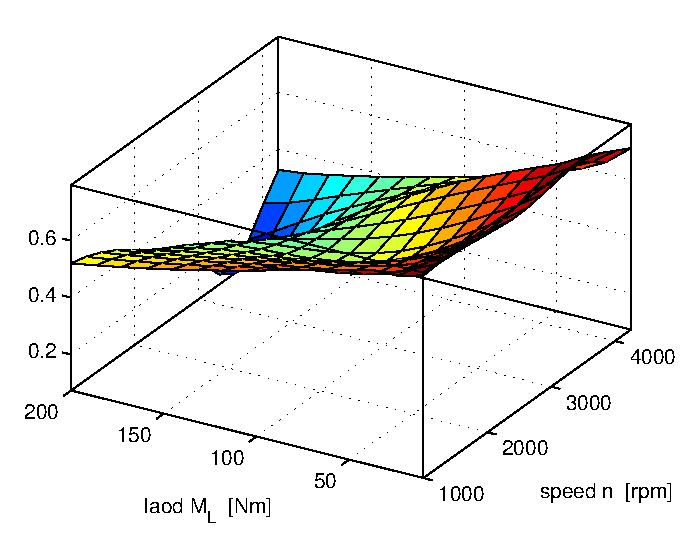
\includegraphics[width=0.75\textwidth]{img/k_surf.eps}
   \caption{Example of a figure.}
   \label{img:k_surf}
\end{figure}
\end{verbatim}

\begin{figure}[ht]
   \centering
   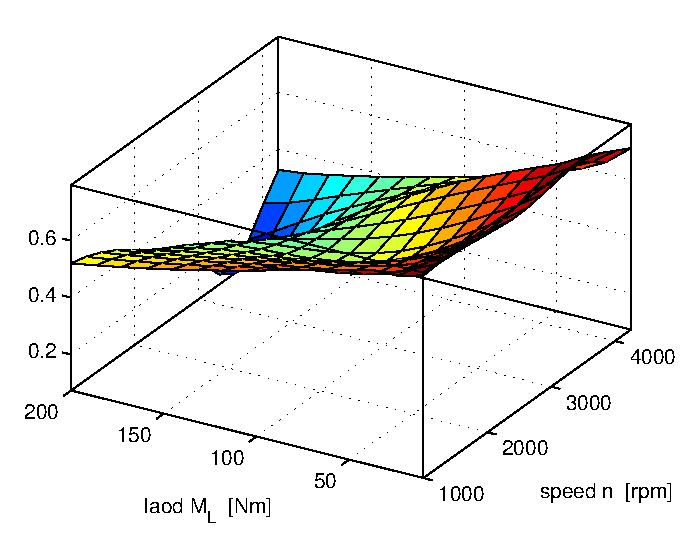
\includegraphics[width=0.75\textwidth]{img/k_surf.eps}
   \caption{Example of a figure.}
   \label{img:k_surf}
\end{figure}

Two figures are displayed next to each other using
\begin{verbatim}
\begin{figure}[ht]
  \begin{minipage}[t]{0.48\textwidth}
    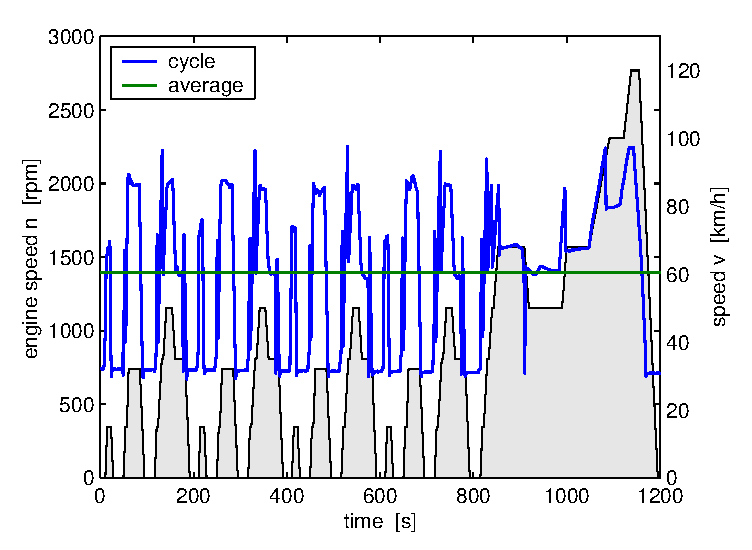
\includegraphics[width = \textwidth]{img/cycle_we.eps}
  \end{minipage}
  \hfill
  \begin{minipage}[t]{0.48\textwidth}
    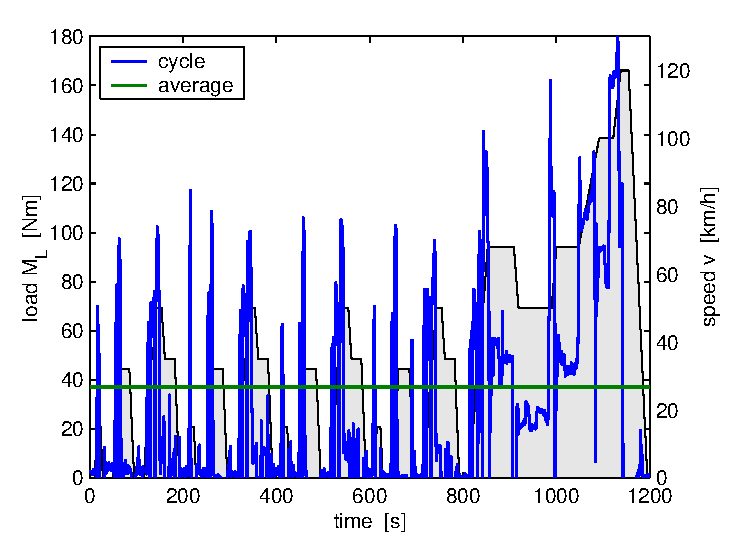
\includegraphics[width = \textwidth]{img/cycle_ml.eps}
  \end{minipage}
  \caption{Two figures next to each other.}
  \label{img:cycle}
\end{figure}
\end{verbatim}

\begin{figure}[ht]
  \begin{minipage}[t]{0.48\textwidth}
    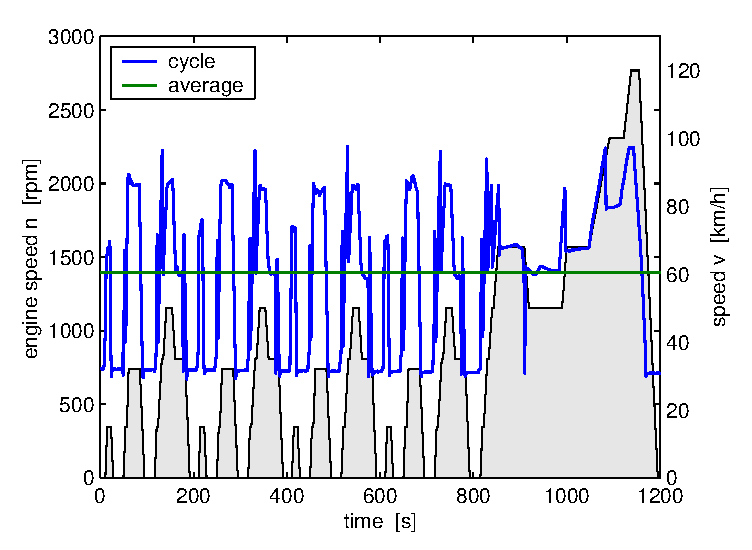
\includegraphics[width = \textwidth]{img/cycle_we.eps}
  \end{minipage}
  \hfill
  \begin{minipage}[t]{0.48\textwidth}
    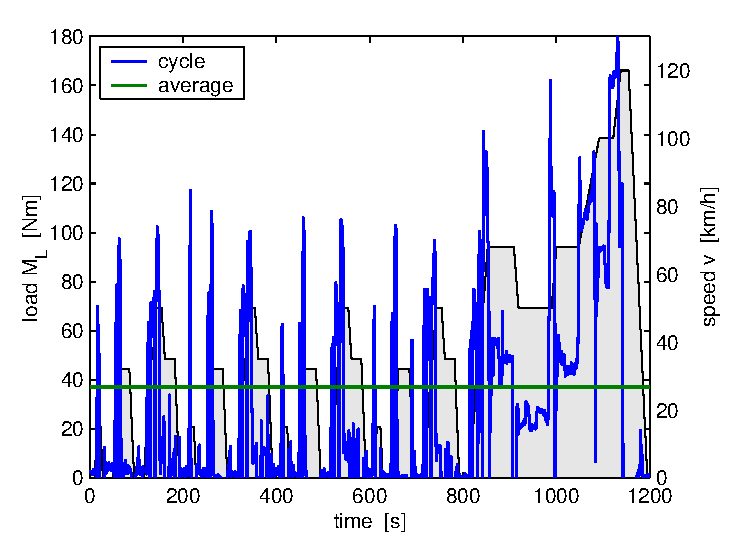
\includegraphics[width = \textwidth]{img/cycle_ml.eps}
  \end{minipage}
  \caption{Two figures next to each other.}
  \label{img:cycle}
\end{figure}

The positioning parameter \texttt{h} (here) forces your figure to be placed in the current position relative to your text. You may add \texttt{t} (top), \texttt{b} (bottom), and/or \texttt{p} (page) to allow for more flexible positioning within your document. For instance, \texttt{[tb]} forces your figure to be placed either on the top or bottom of a page.


\section{Equations}\label{sec:math}
The most common way to include equations is using the \texttt{equation} environment.
\begin{equation}\label{eq:p_me0f}
 p_\mathrm{me0f}(T_e,\omega_e) \ = \ k_1(T_e) \cdot (k_2+k_3 S^2
 \omega_e^2) \cdot \Pi_\mathrm{max} \cdot \sqrt{\frac{k_4}{B}} \, .
\end{equation}
It is recommended to use \texttt{\textbackslash mathrm\{.\}} for subscripts comprising more than two letters since it reduces the width of the subscript significantly and improves readability. The corresponding code is
\begin{verbatim}
\begin{equation}\label{eq:p_me0f}
 p_\mathrm{me0f}(T_e,\omega_e) \ = \ k_1(T_e) \cdot (k_2+k_3 S^2
 \omega_e^2) \cdot \Pi_\mathrm{max} \cdot \sqrt{\frac{k_4}{B}} \, .
\end{equation}
\end{verbatim}
Equations, such as Eq.~\eqref{eq:p_me0f}, may be referenced using \texttt{\textbackslash eqref\{.\}}. In-line mathematical content is created using \texttt{\$.\$}, for example $a^2+b^2=c^2$. It is practically possible to typeset any equation in \LaTeX. Equation~\eqref{eq:advanced} shows an example of a more advance structure.
\begin{equation}\label{eq:advanced}
x^k_n(i) = \left\{\begin{array}{ll}y(i) & \text{if}\quad x^k_{n-1}(i)\leq \mathbf{x}\\
z(i) & \text{otherwise}\end{array}\right., \text{for}\quad i=\{1,\ldots,N\}.
\end{equation}



\section{Including Code in your Document}
Include samples from your Matlab code using the \texttt{lstlistings} environment, for example
\lstset{language=Matlab,numbers=none}
\begin{lstlisting}[frame=lines]
% Evaluate y = 2x
for i = 1:length(x)

  y(i) = 2*x(i);

end
\end{lstlisting}
This example was created using
\begin{verbatim}
\lstset{language=Matlab,numbers=none}
\begin{lstlisting}[frame=lines]
% Evaluate y = 2x
for i = 1:length(x)

  y(i) = 2*x(i);

end
\end{lstlisting}
\end{verbatim}
where \texttt{\textbackslash usepackage\{mcode\}} must be included in the preamble of your document. If you want to include the entire content of a file \texttt{mycode.m} in your document, simply input the path to \texttt{mycode.m} instead of pasting the entire content into your \TeX -file
\begin{verbatim}
\lstset{language=Matlab,numbers=left}
\lstinputlisting{path/to/mycode.m}
\end{verbatim}
Including the path to your m-file also ensures that the code in your report is always up-to-date. The \texttt{\textbackslash lstset\{language=Matlab\}} command ensures that \textsc{Matlab} syntax definitions are used, but many other languages are recognised as well such as \texttt{Fortran} and \texttt{C++}.

%\cleardoublepage
% \input{}
% \cleardoublepage
% \input{}
% \cleardoublepage
% ...

% Appendix______________________________________________________________________
%\appendix
%\chapter{Quantum state preparation routine for Gaussian distributions}\label{sec:stateprepgaussian}

To keep the discussion simple, the task is to load one Gaussian input distribution $R$ and two Gaussian training samples; $L_1$ and $L_2$, such that the amplitude-based kNN algorithm can be used to classify $R$. Note that the input and training distributions are restricted to Gaussian distributions that can be initialized by using the coin gate $C(\delta)$ for some value of $\delta$. The input and training samples all have $N$ entries whereby $N$ is restricted to be a multiple of two. To encode the distributions, $n$ data qubits are required such that there are $2^n = N$ amplitudes. Additionally, one ancilla, one class and one $m$ qubit are needed. Since all qubits are initialised to the \0 state, the initial state is 

\begin{equation}
\ket{\Upsilon_0} = \ket{a;d_1,...,d_n;c;m} = \ket{0;0_1,...,0_n;0;0}
\end{equation}

where the first register holds the ancilla ($a$), the second register contains the $n$ data qubits ($d$) used to encode the distributions and the third and fourth register consists of the class ($c$) and $m$-qubit respectively.

As already demonstrated in Eq.~\ref{equ:chi1} and Eq.~\ref{equ:chi2} in Section~\ref{subsubsec:implementationamplitudeKNN}, the ancilla and $m$-register are each put into an equal superposition through the application of two H gates. The state is then

\begin{equation}
\ket{\Upsilon_1} = \frac{1}{2} \sum_{m=0}^1 \big[ \ket{0}\ket{0_1,...,0_n} + \ket{1}\ket{0_1,...,0_n}\big] \ket{0}\ket{m}
\end{equation}

Suppose the Gaussian distribution $R$ is obtained by choosing $\delta = \tau$ for the coin gate $C(\delta)$. Then the next step is to make use of the controlled version of the coin gate $CC(\tau)$ controlled by the ancilla qubit. $CC(\tau)$ is applied to each of the $n$ qubits in the data register to load the input distribution $R$. Hence, the new quantum state is 

\begin{equation}
\ket{\Upsilon_2} = \prod^n_{j=1} CC(\tau)(a,d_j) \ket{\Upsilon_1} = \frac{1}{2} \sum_{m=0}^1 \big[ \ket{0}\ket{0_1,...,0_n} + \ket{1}\ket{R}\big] \ket{0}\ket{m}
\end{equation}

Since the algorithm is simulated in Liqui$\ket{}$, it is straightforward to define the controlled version of the coin gate $C(\delta)$. 

Next, using an X gate to flip the ancilla moves the input distribution $R$ onto the \0 state of the ancilla such that the state is now

\begin{equation}
\ket{\Upsilon_3} = X(a) \ket{\Upsilon_2} = \frac{1}{2} \sum_{m=0}^1 \big[ \ket{0}\ket{R} + \ket{1}\ket{0_1,...,0_n}\big] \ket{0}\ket{m}
\end{equation}

Suppose the first training distribution $L_1$ can be loaded by choosing $\delta = \sigma$ and applying $C(\sigma)$ to the qubit pattern $\ket{0_1,...,1_5,0_6,...,0_n}$. Thus, the fifth qubit in the data register connected to the \1 ancilla state needs to flipped into the \1 state. This can be done with a CCNOT gate, controlled by the ancilla and $m$ qubit, acting on the fifth data qubit. Next, by applying the controlled controlled version of the coin gate $CCC(\sigma)$ to each data qubit controlled by the ancilla and the $m$ qubit the training sample $L_1$ is loaded. The quantum state is then given by
\begin{align}
\ket{\Upsilon_4} &= \prod^n_{j=1} CCC(\sigma)(a,m,d_j) CCNOT(a,m,d_5) \ket{\Upsilon_3}\notag\\
&= \frac{1}{2} \Big[\big[ \ket{0}\ket{R} + \ket{1}\ket{0_1,...,0_n}\big] \ket{0}\ket{0} + \big[\ket{0}\ket{R} + \ket{1}\ket{L_1*}\big] \ket{0}\ket{1}\Big]
\end{align}

Since the last entry on the diagonal of the coin gate (see Eq.~\ref{equ:coingate}) is negative, the application of $CCC(\sigma)$ introduces a negative sign when applied to the fifth data qubit. Hence, not the exact distribution $L_1$ but a distribution $L_1^*$ with a sign difference was loaded into $\ket{\Upsilon_4}$. As explained in Section~\ref{subsec:amplitudeKNNalgorithm}, the amplitude-based kNN algorithm makes use of interference between the input and training samples whereby the negative sign would alter the outcome of the interference. Thus, the sign needs to be corrected by acting a controlled controlled Z gate on the fifth data qubit. Thereafter, the $m$ qubit is flipped with an X gate to move $L_1$ onto the \0 state of the $m$ qubit. After these gate operations the state is
\begin{align}
\ket{\Upsilon_5} &= X(m) CCZ(d_5) \ket{\Upsilon_4}\notag\\
&= \frac{1}{2} \Big[\big[ \ket{0}\ket{R} + \ket{1}\ket{L_1}\big] \ket{0}\ket{0} + \big[\ket{0}\ket{R} + \ket{1}\ket{0_1,...,0_n}\big] \ket{0}\ket{1}\Big]
\end{align}

For the second training distribution $L_2$, suppose it results from choosing $\delta = \nu$ and applying $C(\nu)$ to the qubit pattern $\ket{1_1,...,1_n}$. Thus, all data qubits connected to the \1 ancilla and \1 $m$-qubit state have to be flipped using a CCNOT gates. As outlined in the previous step, $CCC(\nu)$ loads the distribution $L_2^*$ and not $L_2$ because of sign differences. Since all data qubits are \1, these signs are corrected by acting controlled controlled Z gates on all data qubits controlled by the ancilla and $m$-qubit. The state containing the input and both training distributions is then

\begin{align}
\ket{\Upsilon_6} &= \prod^n_{j=1} CCZ(d_j) CCC(\sigma)(a,m,d_j) CCNOT(a,m,d_j) \ket{\Upsilon_5}\notag\\
&= \frac{1}{2} \Big[\big[ \ket{0}\ket{R} + \ket{1}\ket{L_1}\big] \ket{0}\ket{0} + \big[\ket{0}\ket{R} + \ket{1}\ket{L_2}\big] \ket{0}\ket{1}\Big]
\end{align}

Lastly, the class qubit for $L_2$ is flipped with a CNOT gate controlled by the $m$ qubit such that the final state is
\begin{align}
\ket{\Upsilon_6} &= CNOT(m,c) \ket{\Upsilon_6}\notag\\
&= \frac{1}{2} \Big[\big[ \ket{0}\ket{R} + \ket{1}\ket{L_1}\big] \ket{0}\ket{0} + \big[\ket{0}\ket{R} + \ket{1}\ket{L_2}\big] \ket{1}\ket{1}\Big]
\end{align}


$\ket{\Upsilon_7}$ is in the form of the initial quantum state (Eq.~\ref{equ:ampinitial}) required for the amplitude-based kNN algorithm. This completes the quantum state preparation routine for loading a restricted subset of discrete Gaussian distributions using the coin gate $C(\delta)$.

 \cleardoublepage



% Bibliography__________________________________________________________________
% Literature (Additional references can be added to the .bib-file manually, or by using, for example, the free application JabRef). Compile in the following order: latex -bibtex -latex -latex

\bibliographystyle{apacite}
\bibliography{thesis}

\end{document}
